%%%%%%%%%%%%%%%%%%%%%%%%%%%%%%%%%%%%%%%%%
% Short Sectioned Assignment
% LaTeX Template
% Version 1.0 (5/5/12)
%
% This template has been downloaded from:
% http://www.LaTeXTemplates.com
%
% Original author:
% Frits Wenneker (http://www.howtotex.com)
%
% License:
% CC BY-NC-SA 3.0 (http://creativecommons.org/licenses/by-nc-sa/3.0/)
%
%%%%%%%%%%%%%%%%%%%%%%%%%%%%%%%%%%%%%%%%%

%----------------------------------------------------------------------------------------
% PACKAGES AND OTHER DOCUMENT CONFIGURATIONS
%----------------------------------------------------------------------------------------

\documentclass[paper=a4, fontsize=11pt]{scrartcl} % A4 paper and 11pt font size

\usepackage[T1]{fontenc} % Use 8-bit encoding that has 256 glyphs
\usepackage{fourier} % Use the Adobe Utopia font for the document - comment this line to return to the LaTeX default
\usepackage[norsk]{babel} 
\usepackage[utf8]{inputenc}
\usepackage{amsmath,amsfonts,amsthm} % Math packages
\usepackage{tikz} % drawing package

\usepackage{sectsty} % Allows customizing section commands
\allsectionsfont{\centering \normalfont\scshape} % Make all sections centered, the default font and small caps

\usepackage{fancyhdr} % Custom headers and footers
\pagestyle{fancyplain} % Makes all pages in the document conform to the custom headers and footers
\fancyhead{} % No page header - if you want one, create it in the same way as the footers below
\fancyfoot[L]{} % Empty left footer
\fancyfoot[C]{} % Empty center footer
\fancyfoot[R]{\thepage} % Page numbering for right footer
\renewcommand{\headrulewidth}{0pt} % Remove header underlines
\renewcommand{\footrulewidth}{0pt} % Remove footer underlines
\setlength{\headheight}{13.6pt} % Customize the height of the header

\numberwithin{equation}{section} % Number equations within sections (i.e. 1.1, 1.2, 2.1, 2.2 instead of 1, 2, 3, 4)
\numberwithin{figure}{section} % Number figures within sections (i.e. 1.1, 1.2, 2.1, 2.2 instead of 1, 2, 3, 4)
\numberwithin{table}{section} % Number tables within sections (i.e. 1.1, 1.2, 2.1, 2.2 instead of 1, 2, 3, 4)

\setlength\parindent{0pt} % Removes all indentation from paragraphs - comment this line for an assignment with lots of text

%---- Listings --------------
\usepackage{color}
\definecolor{light-gray}{gray}{0.95}
\usepackage{listings}

\lstnewenvironment{code}[1][]%
{\minipage{\linewidth}
\lstset{ %
language={[x86masm]Assembler},  % choose the language of the code
basicstyle=\footnotesize,       % the size of the fonts that are used for the code
numbers=left,                   % where to put the line-numbers
numberstyle=\footnotesize,      % the size of the fonts that are used for the line-numbers
stepnumber=1,                   % the step between two line-numbers. If it is 1 each line will be numbered
resetmargins=true,              % reset line numbers
numbersep=5pt,                  % how far the line-numbers are from the code
backgroundcolor=\color{white},  % choose the background color. You must add \usepackage{color}
showspaces=false,               % show spaces adding particular underscores
showstringspaces=false,         % underline spaces within strings
showtabs=false,                 % show tabs within strings adding particular underscores
frame=single,                   % adds a frame around the code
tabsize=2,                      % sets default tabsize to 2 spaces
captionpos=b,                   % sets the caption-position to bottom
breaklines=true,                % sets automatic line breaking
breakatwhitespace=false,        % sets if automatic breaks should only happen at whitespace
escapeinside={\%*}{*)},         % if you want to add a comment within your code
morekeywords={
    orr, ldr, bne, subs
    },                          % additional keywords to expand the asm language
#1
}}%
{\endminipage}

%----------------------------------------------------------------------------------------
% TITLE SECTION
%----------------------------------------------------------------------------------------

\newcommand{\horrule}[1]{\rule{\linewidth}{#1}} % Create horizontal rule command with 1 argument of height

\title{ 
\normalfont \normalsize 
\textsc{TDT4205 Compilers, NTNU} \\ [25pt] % Your university, school and/or department name(s)
\horrule{0.5pt} \\[0.4cm] % Thin top horizontal rule
\huge Problem Set 6 \\ % The assignment title
\horrule{2pt} \\[0.5cm] % Thick bottom horizontal rule
}

\author{Christoffer Tønnessen} % Your name

\date{\normalsize27. march 2014} % Today's date or a custom date

\begin{document}

\maketitle % Print the title

%----------------------------------------------------------------------------------------
% PROBLEM 1
%----------------------------------------------------------------------------------------
\section{Optimalization 1}

%----------------------------------------------------------------------------------------
\subsection{Part a)}
In common subexpression elimination the notion is to not compute a value twice.
When something is computed one would want to not recompute this again.
There are two variants, which is local common-subexpression and global common-subexpression.
The latter looks at the whole system and where one can find already calculated values, while the other one looks at a block isolated.

In our case one can observe that $ i + t $ is calculated twice.
Though this is not a viable place to optimize, since the result is again saved in $i$.
So the second $i$ is different from the first one.

We can not do anything in this step for our flow graph.

%----------------------------------------------------------------------------------------
\subsection{Part b)}
In copy propagation the idea is that when $ u = v $ occures, one want to use v for u all the time afterwards.
This in itself might not seem so very useful, but it will give the opportunity to eliminate assignments later on.

We can clearly see that we have $ j = i $ in our block B3. We can now change $j$ with the value $i$ in the expression later $ d = j + 2 $.

%----------------------------------------------------------------------------------------
\subsection{Part c)}
Code motion opts to reduce the operations happening inside a loop.
It is very expensive to do calculations and if some are not neccessary they should not be done over and over again.

The calculation $t = a * c$ will stay the same for the duration of the loop.
This means we can move this calculation up to B1 to avoid having to calculate it every time we do the loop.

%----------------------------------------------------------------------------------------
\subsection{Part d)}
If a variable is not used by the program, it is concidered dead.
It can then be removed completely from the program and it will not alter the behaviour.
This means that the program can be smaller and do an operation less.

After we delcare $ d = 0 $ the value of $d$ is not read before $ d = j + 2 $.
This means that we can remove the line $ d = 0 $.

%----------------------------------------------------------------------------------------
\subsection{Extra}
There are a lot of variables in B3 which we can not see the context of.
Some of these might be unneccessary if seen in a bigger picture.
If B4 returns nothing the whole B2 and B3 loop could be optimized to have a certan number of $nop$ operations.

%----------------------------------------------------------------------------------------
% PROBLEM 2
%----------------------------------------------------------------------------------------
\section{Optimization 2}

%----------------------------------------------------------------------------------------
\subsection{Part a)}
An induction variable is a variable which has a constant $c$ such that each time that variable is assigned, its value is increased by $c$.
This is something that happens a lot when one is talking about loops and counters of that loop.
There are a lot of room to optimize that variable as one can assume a program will have a lot of variables on that form.

Reduction in strength is the transformation of replacing an expensive operation with a less expensive operation.
One example of this is to change multiplication with addition, as addition is much cheaper than multiplication.

These two things are tightly linked together as one can usually reduce the strength of an induction variable and then optimize your program's speed and make it smaller.

%----------------------------------------------------------------------------------------
\newpage
\subsection{Part b)}
\begin{figure}[ht!]
\centering
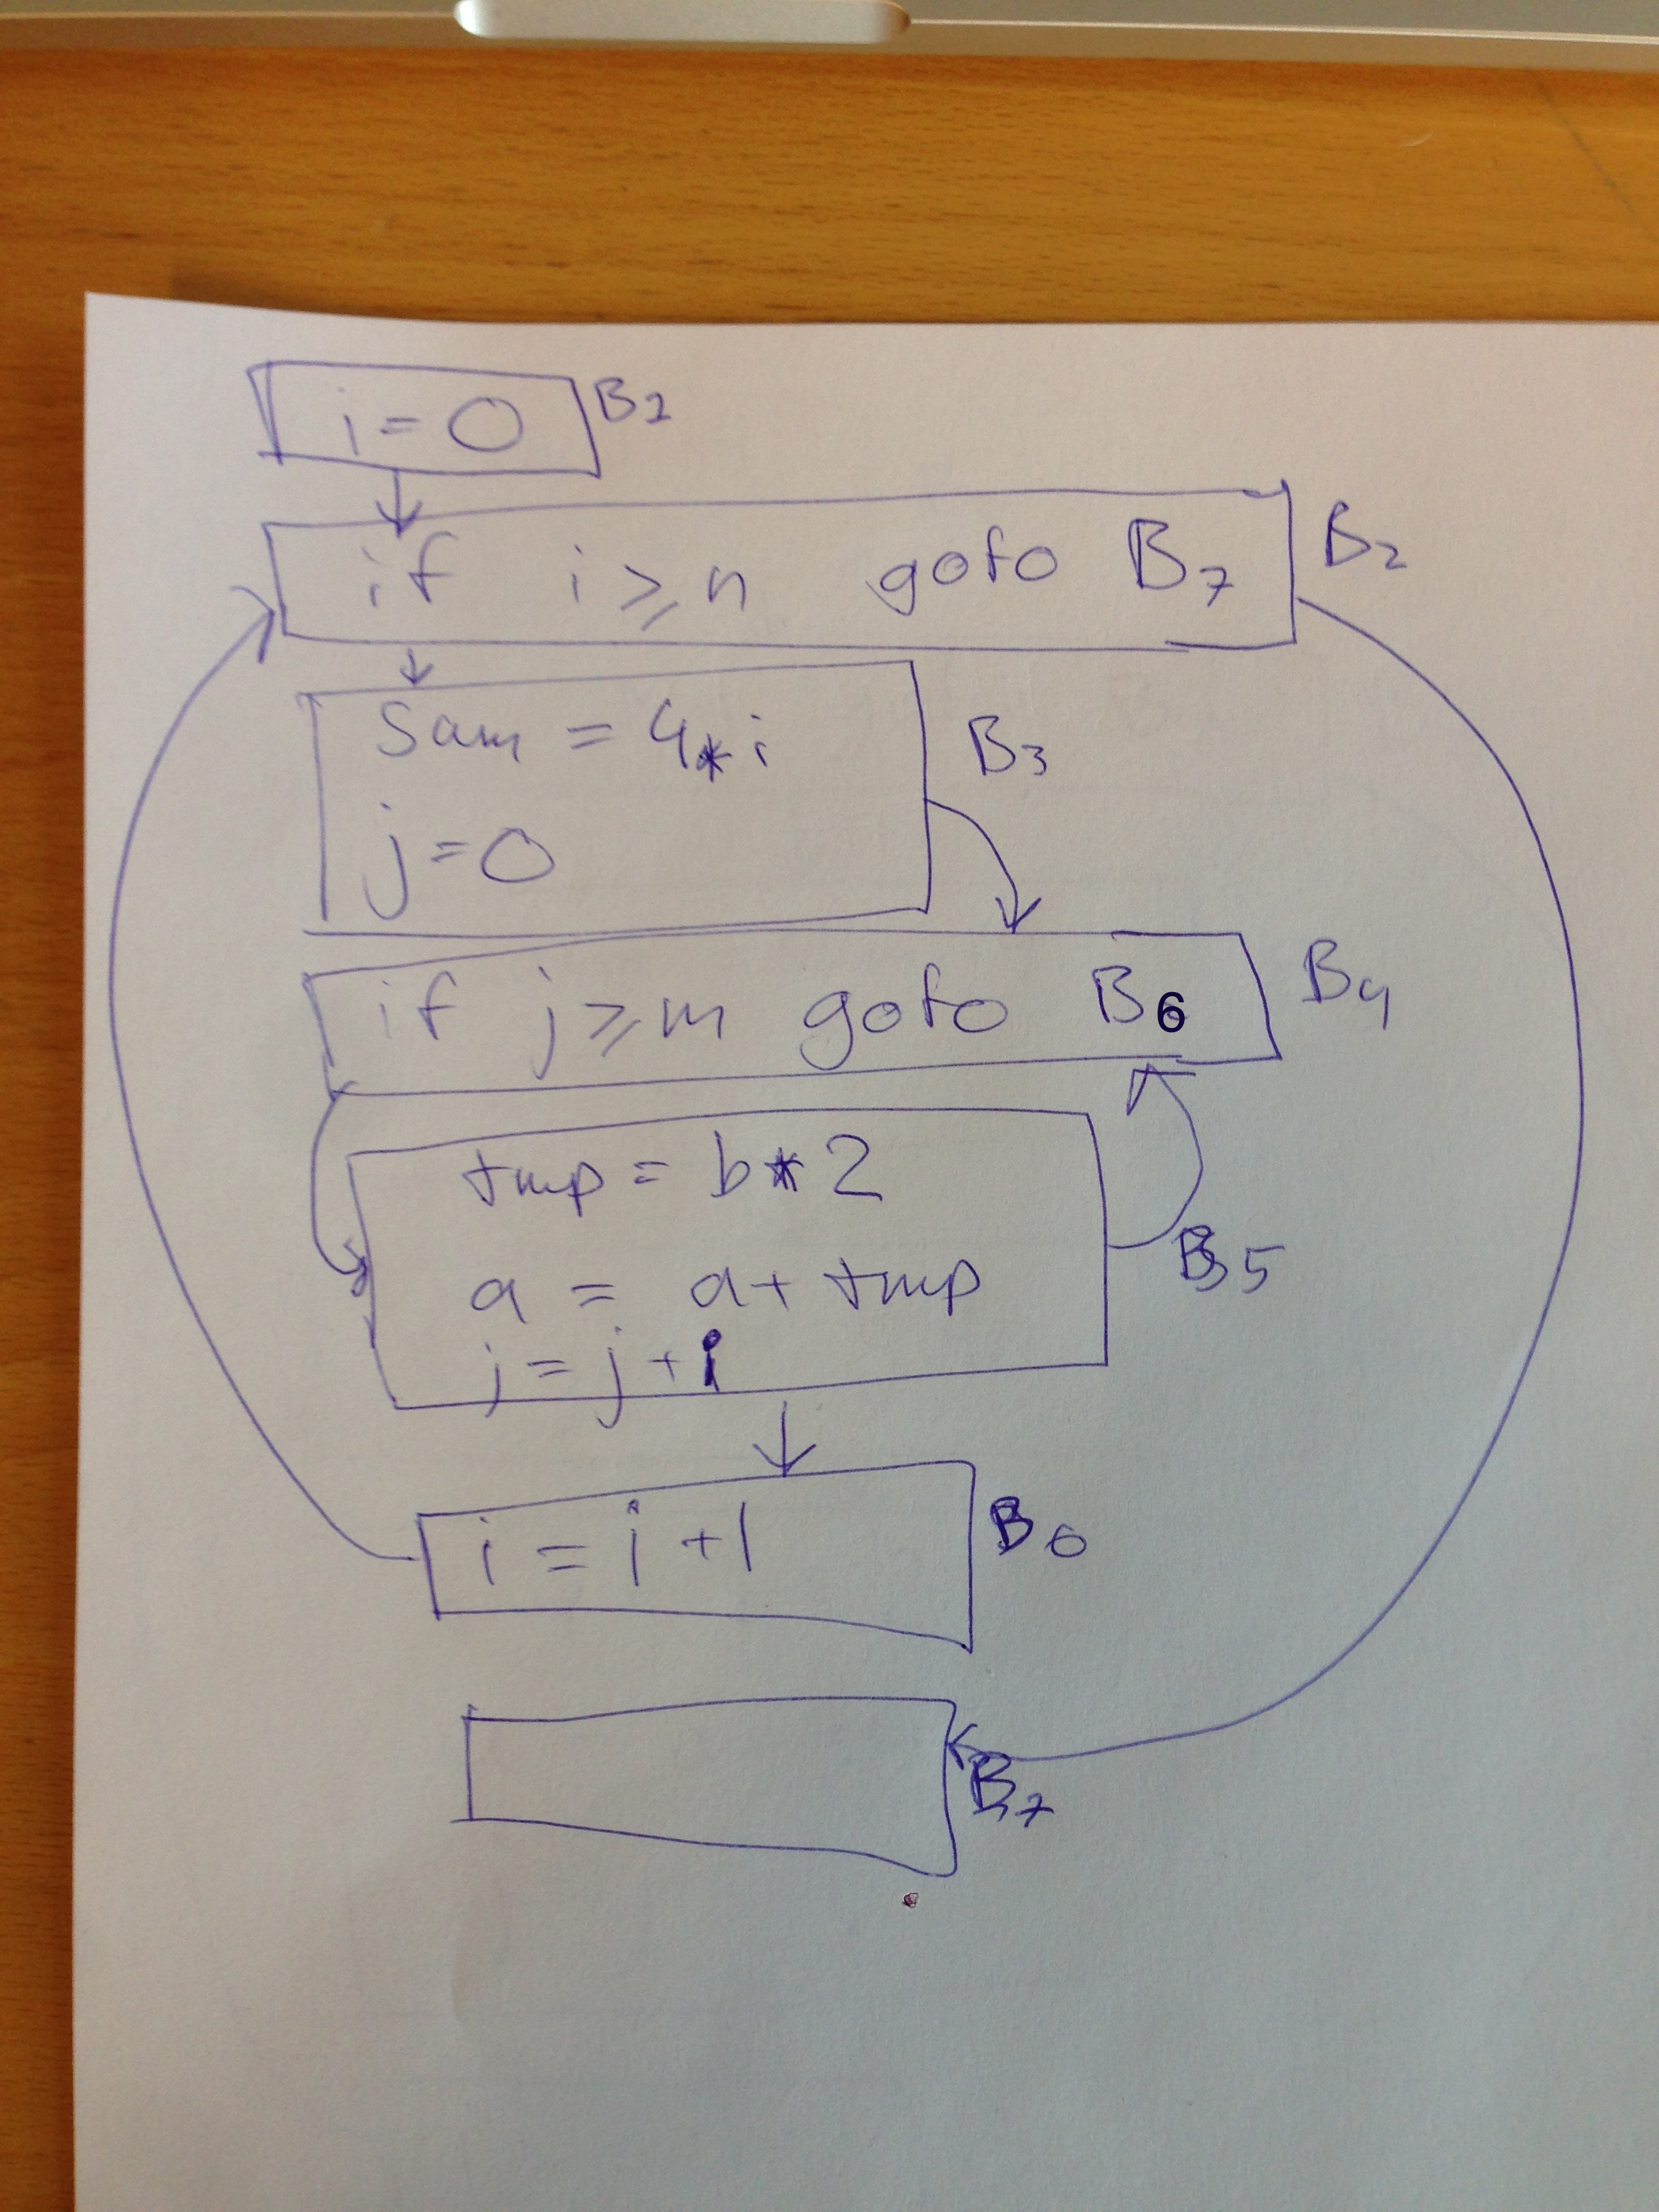
\includegraphics[width=80mm]{2b.jpg}
\caption{Code as a three-adress flow graph}
\label{fig:2b}
\end{figure}

%----------------------------------------------------------------------------------------
\newpage
\subsection{Part c)}
\begin{figure}[ht!]
\centering
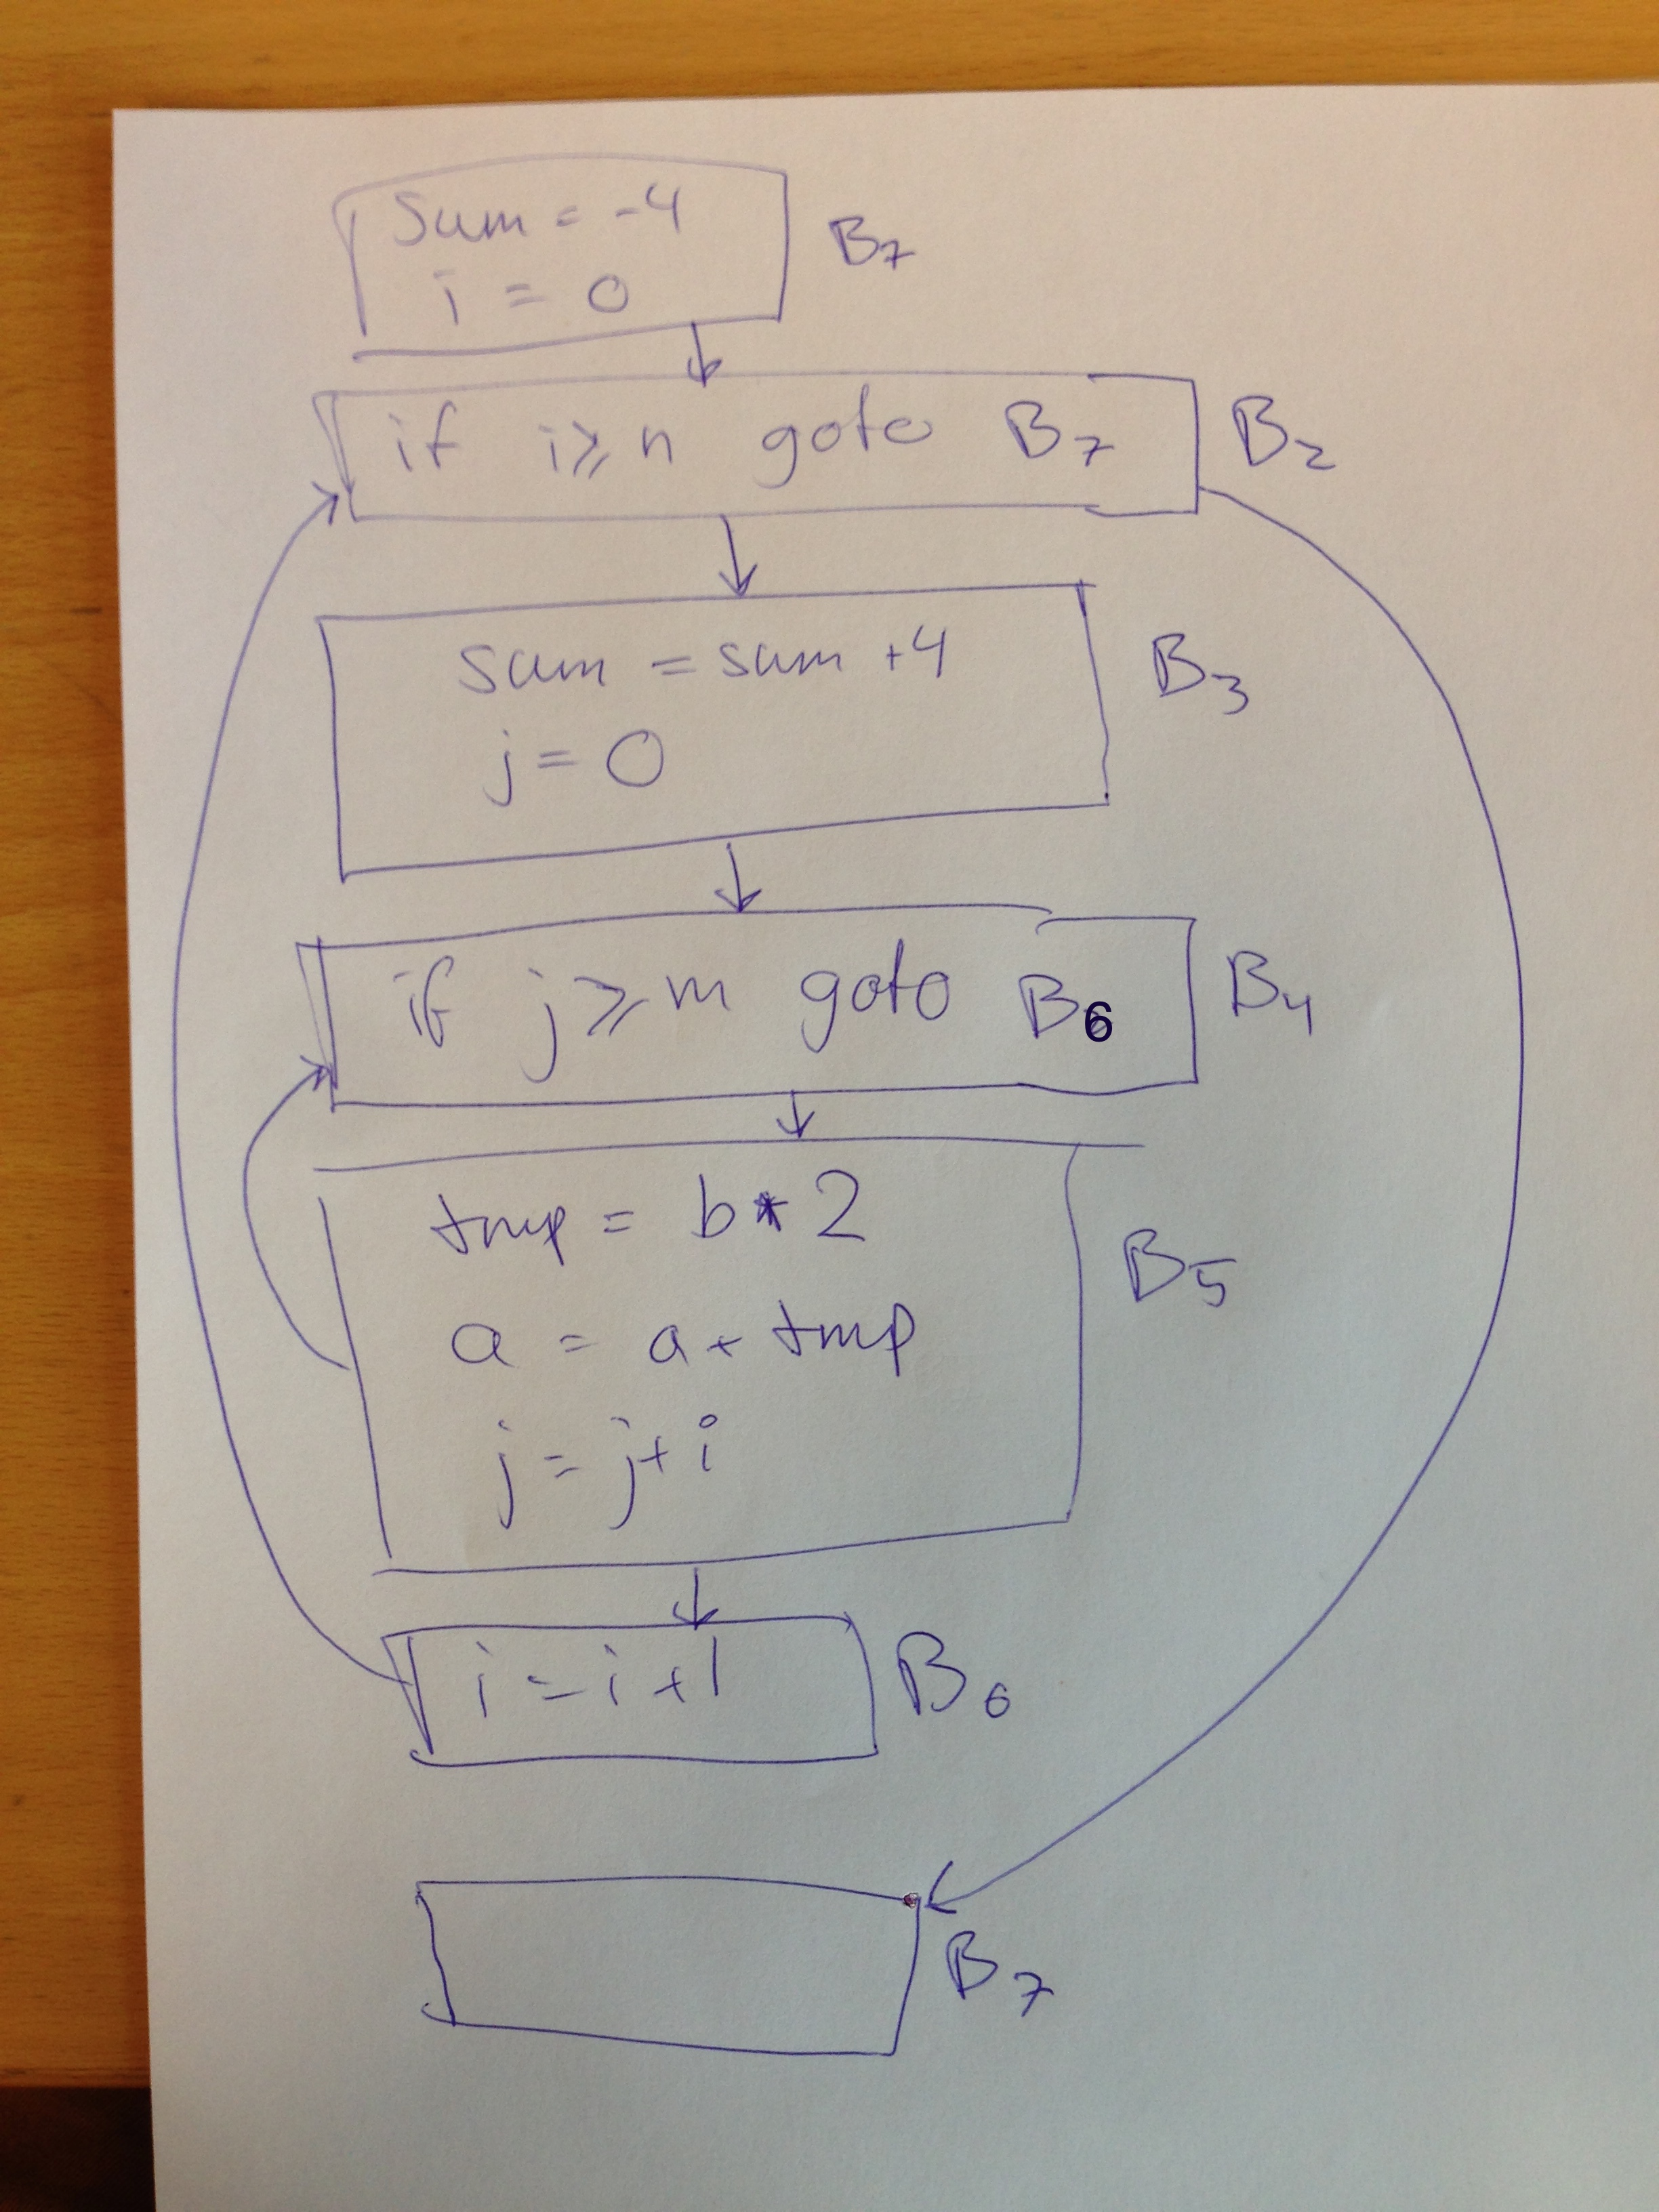
\includegraphics[width=80mm]{2c.jpg}
\caption{Optimized 2b with strength reduction}
\label{fig:2c}
\end{figure}

%----------------------------------------------------------------------------------------
% PROBLEM 3
%----------------------------------------------------------------------------------------
\section{Data-flow analysis}

%----------------------------------------------------------------------------------------
\subsection{Part a)}
The reach of a definition is all the points in the code where one can be sure that the definition stays the same and is not changed.
This requirement must be met at compile time.
This means that if you can branch two ways at one point in your program, both branches must be taken into concideration.

Take the flow graph from problem 3.
The reach for the variable $f$ given that it's defined somewhere before our entry is $d9$.
We know this because the variable is altered in $d7$.
Because of the branching from B2 we will not know at compile time when we enter $d10$ which branch we took.
Therefor the points in which we have a reach is $d1$ to $d9$.

%----------------------------------------------------------------------------------------
\newpage
\subsection{Part b)}
After two iterations we see that B5 has the same in and out set.
This means that the set has converged and is now correct in all states.

\begin{table}[ht!]
    \begin{tabular}{|p{1cm}|p{2cm}|p{2cm}|p{2cm}|p{2.1cm}|p{2cm}|p{2.1cm}|}
    \hline
    Block & Gen           & Kill                      & In - round 1               & Out - round 1                     & In - round 2                      & Out - round 2                     \\ \hline
    B1    & d1, d2, d3    & d5, d6, d8, d10, d11, d12 & empty                      & d1, d2, d3                        & d4, d6, d7, d8, d9, d10, d11, d12 & d1, d2, d3, d4, d7, d9            \\ \hline
    B2    & d4, d5        & d1, d10                   & d1, d2, d3, d4, d5         & d4, d5, d2, d3                    & d1, d2, d3, d4, d7, d9            & d4, d5, d2, d3, d7, d9            \\ \hline
    B3    & d6, d7        & d2, d8                    & d2, d3, d4, d5             & d6, d7, d3, d4, d5                & d2, d3, d4, d5, d7, d9            & d6, d7, d3, d4, d5, d9            \\ \hline
    B4    & d8, d9        & d2, d6                    & d2, d3, d4, d5             & d8, d9, d3, d4, d5                & d2, d3, d4, d5, d7, d9            & d8, d9, d3, d4, d5, d7            \\ \hline
    B5    & d10, d11, d12 & d1, d3, d5                & d3, d4, d5, d6, d7, d8, d9 & d10, d11, d12, d4, d6, d7, d8, d9 & d3, d4, d5, d6, d7, d8, d9        & d10, d11, d12, d4, d6, d7, d8, d9 \\ \hline
    \end{tabular}
\end{table}
%----------------------------------------------------------------------------------------
\subsection{Part c)}
Observing that both $d6$ and $d8$ is in the out set of B5.
These are the only two places where the b variable is assigned.
This means that one of these two actions must take place.
Therefor we can draw the conclusion that the variable $b$ must be a constant.

%----------------------------------------------------------------------------------------
% PROBLEM 4
%----------------------------------------------------------------------------------------
\section{Register allocation}

%----------------------------------------------------------------------------------------
\subsection{Part a)}
A live variable analysis is a backwards analysis in respect to the flow of the program.
For a variable to be live it means that at a point $p$ the variable could be used along a path from $p$.
If not it's dead.

Let's say we have a variable which at some point $a$ gets written to and at a point $b$ gets read, after some while it gets written to again at a point $c$.
In the time between point $b$ and point $c$, the variable would be dead.
There would be no point in having that variable there at all, and if needed the variable could be deleted.

%----------------------------------------------------------------------------------------
\newpage
\subsection{Part b)}
\begin{table}[ht!]
    \begin{center}
    \begin{tabular}{|l|l|}
    \hline
    Line      & Live variables \\ \hline
    a = a + b & \{ d, a, b, c \} \\ \hline
    d = a + b & \{ d, a, b, c \} \\ \hline
    e = 2 * a & \{ d, a, c \}  \\ \hline
    a = e + c & \{ d, a, e, c \} \\ \hline
    b = d + a & \{ d, a, e \}  \\ \hline
    c = e - 2 & \{ e \}        \\ \hline
    \end{tabular}
    \caption{Live variable analysis for the three address code}
    \end{center}
\end{table}

%----------------------------------------------------------------------------------------
\subsection{Part c)}
\begin{figure}[ht!]
\centering
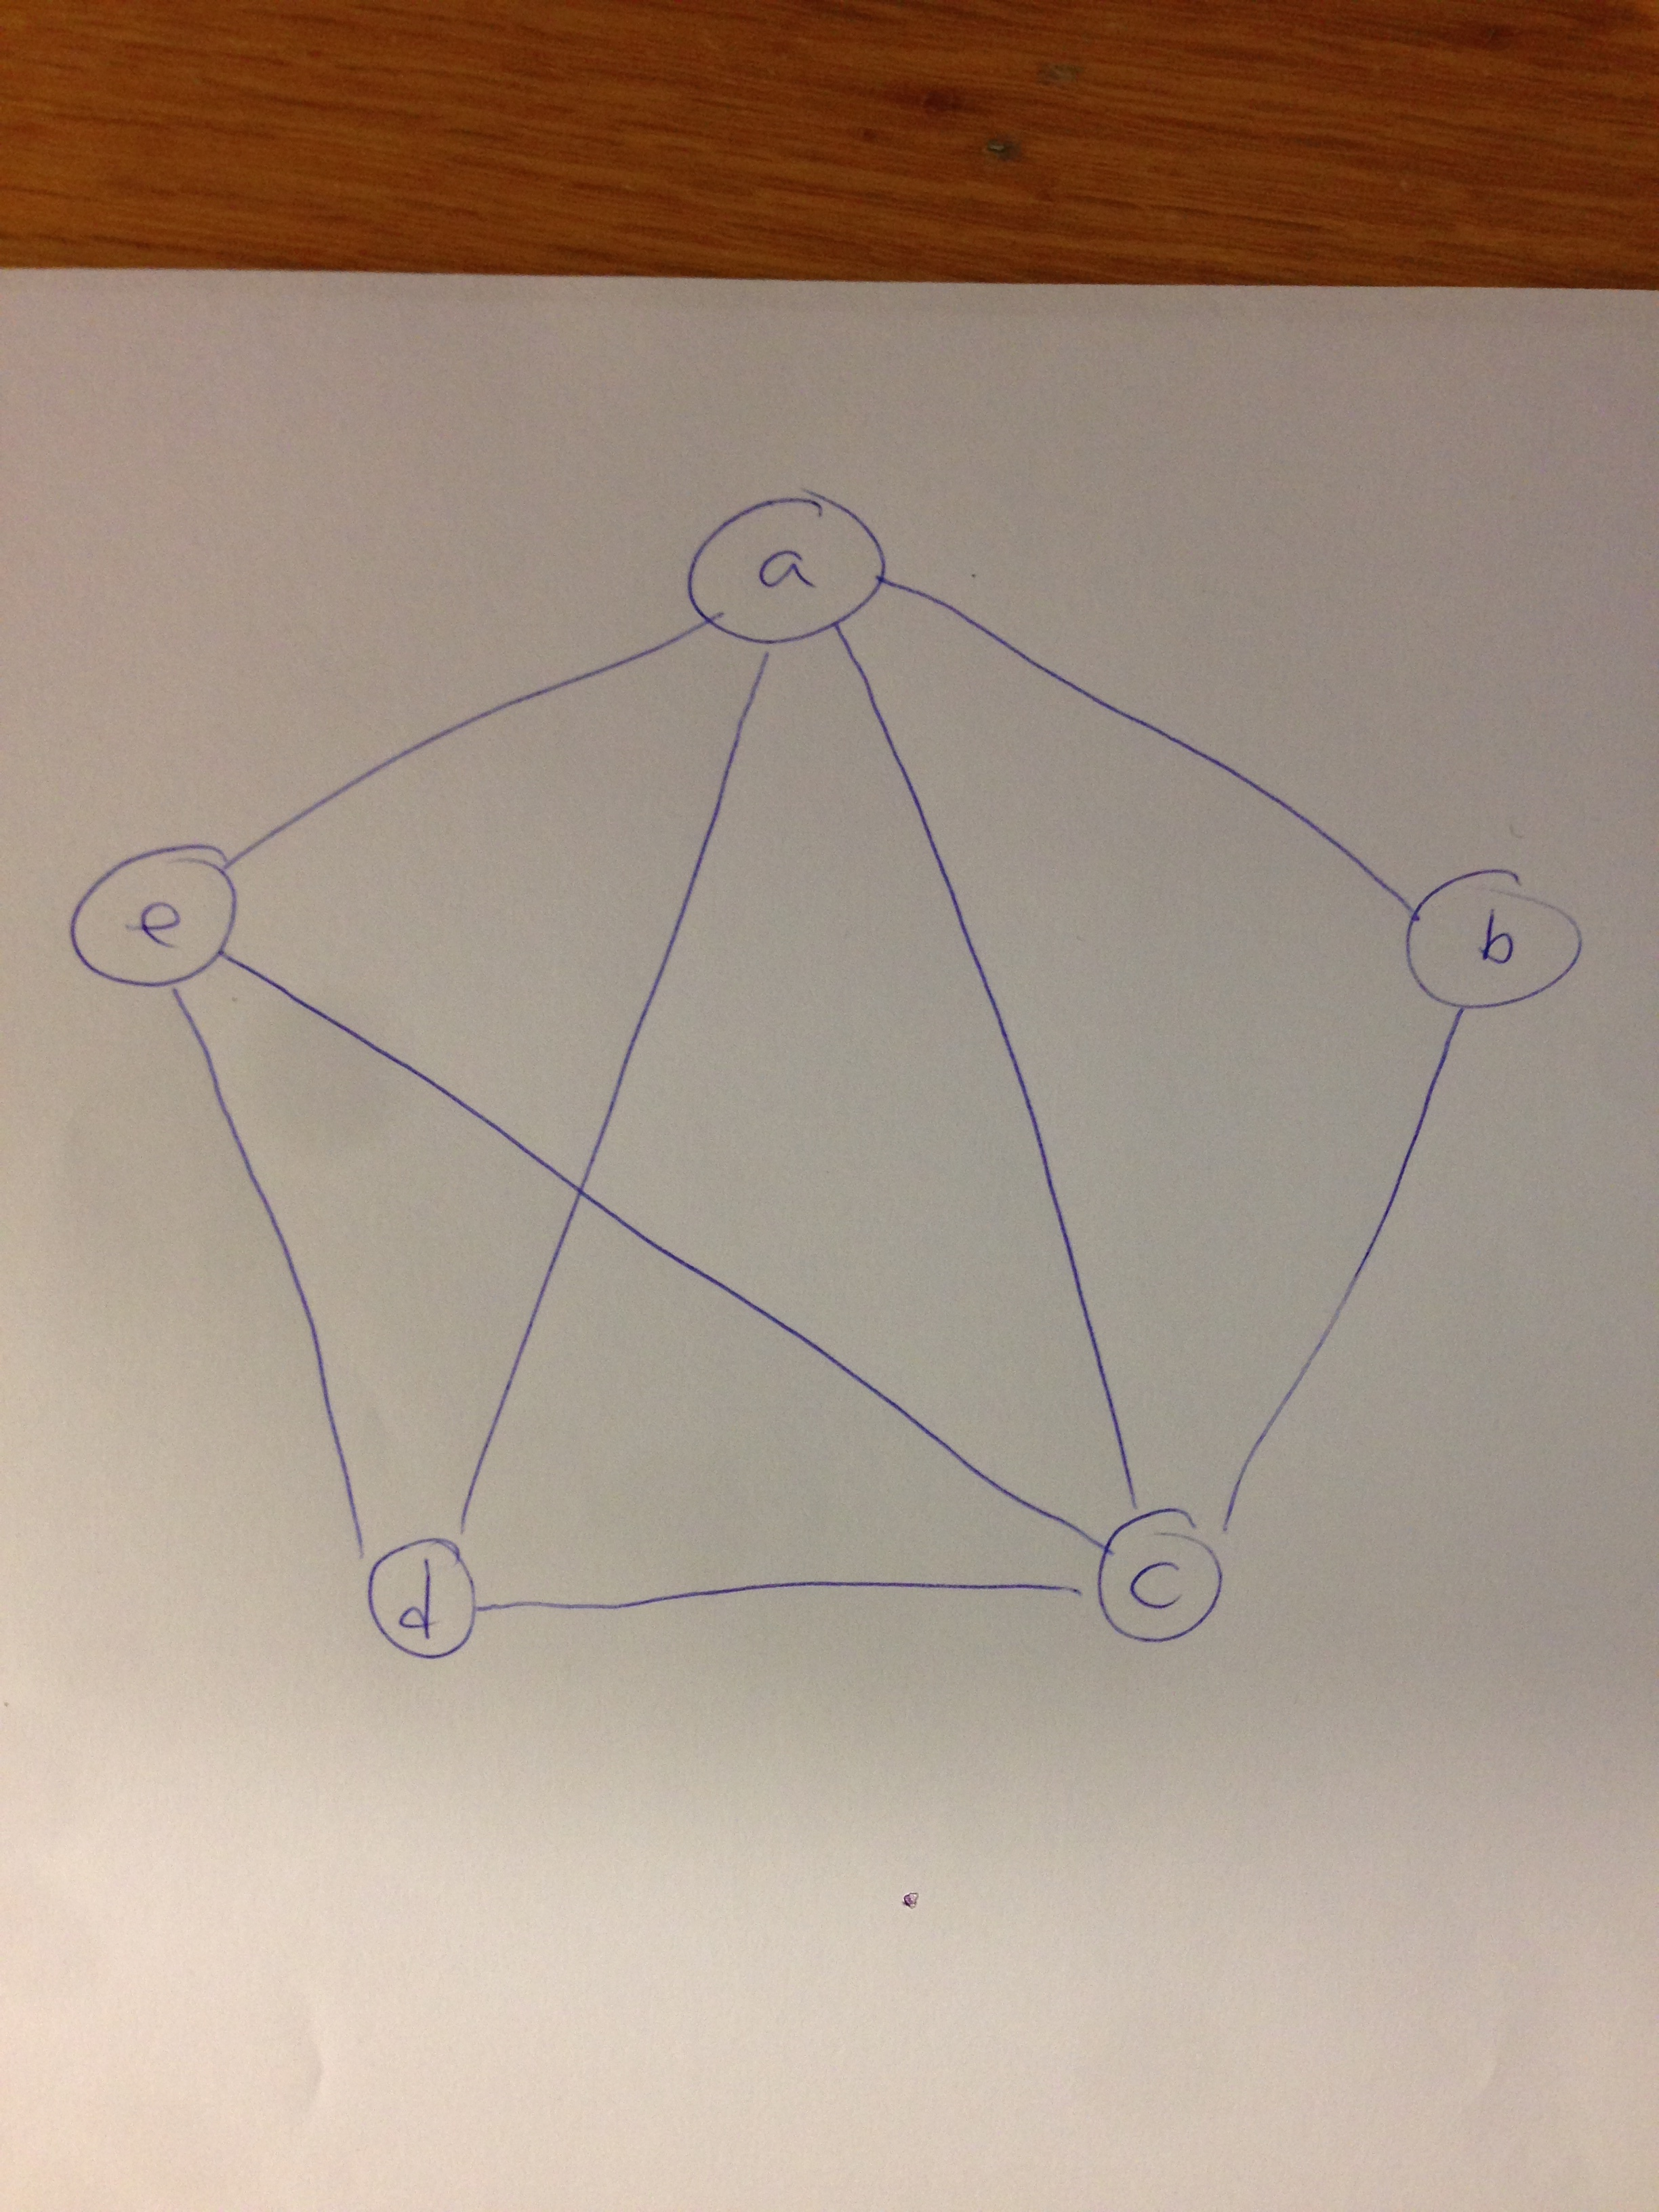
\includegraphics[width=80mm]{4c.jpg}
\caption{Interface graph for the code in Problem 4}
\label{fig:2c}
\end{figure}

%----------------------------------------------------------------------------------------
\subsection{Part d)}
When observing the graph above one can see that $d$ and $b$ is not connected.
To make sure that we avoid register spills we would need to have 4 registers.
Two of the variables which does not share an edge would need to share a register.

%----------------------------------------------------------------------------------------
\end{document}
